\documentclass{article}
\usepackage[utf8]{inputenc} % allows for non-ASCII characters
\usepackage[x11names]{xcolor}    % Color extensions
\usepackage[margin=1in]{geometry} % Formatting on page
\usepackage{array} % big arrays
\usepackage{amsmath} % Math symbols
\usepackage{amsthm}   
\usepackage{amssymb}
\usepackage[backend=bibtex]{biblatex} % bibliography
\usepackage{bm} % bold for greek letters
\usepackage{cancel}
\usepackage[format=hang]{caption}
\usepackage{enumitem} % Enumerating things
\usepackage{esint} % better double and triple Integrals
\usepackage{etoc}
\usepackage{fancyhdr} % Headers
    \pagestyle{fancy}
\usepackage{float}
\usepackage{gensymb}
\usepackage{physics} % easier commands for physics things
\usepackage{relsize}  % allows for larger/smaller math 
\usepackage{textcomp} % Gets rid of perthousand error
\usepackage{upquote}  % fixes quotes in verbatim environment
\usepackage{verbatim} % Allows for comment environment
\usepackage{tikz} % pictures
	\usetikzlibrary{calc}
	\usetikzlibrary{decorations.markings}
	\usetikzlibrary{3d}
	\usetikzlibrary{intersections}
\usepackage{pgfplots} % plots and graphics
	\pgfplotsset{compat=newest} % or use compat=1.6
	\usepgfplotslibrary{fillbetween}
\usepackage{graphicx} % plots and graphics
\usepackage{wrapfig}
\usepackage{xparse} % Better commands
\usepackage[hidelinks]{hyperref}% References--THIS GOES LAST

% Packages that this breaks without: amsmath, gensymb, physics, hyperref, xcolor, xparse, and possibly others
\numberwithin{equation}{section} % amsmath command that renews equation counter in each section\
\def\ints{\int_\mathcal{S}} % Surface integral
\def\intv{\int_\mathcal{V}} % Volume integral with V subscript
\def\intall{\int_{-\infty}^{\infty}} % Integral over all space
\def\iintall{\iint_{\rm All Space}} % Integral over all space
\def\iiintall{\iiint_{\rm All Space}} % Integral over all space
\def\ik{4\pi\epsilon_0} % Inverse k for EM
\def\lap{\mathcal{L}}
\def\answerline{ % double horizontal line placed 0.5 cm below text, space between lines is 0.07 cm, then 0.75 cm of space 
	\vspace{0.5 cm}
	\hrule
	\vspace{0.07 cm}
	\hrule
	\vspace{0.75 cm}\noindent} % don't indent text after the line
\NewDocumentCommand\length{O{3pt}}{\setlength\jot{#1}} % for align vertical spacing, there's probably a better way to do this locally
\NewDocumentCommand\ft{s O{n} O{L}}{ % I dont want to write \sin(stuff) \cos(stuff) every time in fourier transforms (ft)
    \IfBooleanTF{#1}{
        \sin(\frac{#2 \pi}{#3}x)
    }{
        \cos(\frac{#2 \pi}{#3}x)
    }
}

\NewDocumentCommand\dl{s}{\IfBooleanTF{#1}{}{\cdot} d\mathbf{l}} % quicker curve integral dl, if no star, it also makes the dot 
\NewDocumentCommand\da{s}{\IfBooleanTF{#1}{}{\cdot} d\mathbf{a}} % quicker surface integral da, if no star, it also makes the dot 
\NewDocumentCommand\oo{O{1} m} {\frac{#1}{#2}}   % reciprocal- 'one over', option to make it a regular fraction because oo is still quicker to type.
\NewDocumentCommand\thetitle{m O{}}{ \title{ \hypertarget{top}{\textbf{#1}} \\ \large {#2} } } %Bold title that is a hypertarget, optional bolded subtitle that's scaled properly 

\NewDocumentCommand \e {s m}{ % basis vector command
	\IfBooleanTF{#1} % \e{x} for x hat notation, \e*{x} for e_x notation
	{\mathbf{\hat{e}_{#2}}}
	{\bm{\hat{#2}}}} % from package bm, more powerful than \mathbf} 
\NewDocumentCommand \parametric {m}{ %command for getting boundary conditions with a "{" on the left
    \left\{ 
	\begin{gathered}
		\begin{matrix}
			#1
    		\end{matrix}
	\end{gathered}
	 \right.}
\NewDocumentCommand \der {s O{} m g}{ % custom derivative command
     \IfBooleanTF{#1} % if \der*, #1 is true, euler notation used, if \der , #1 is false, d/dx is used 
    {\IfNoValueTF{#4}  % g returns -NoValue- if no argument (read below)
        {\mathrm{D}_{#3}^{#2}}  % g is included so \der{x} and \der{f}{x} both have x in the denominator
        {\mathrm{D}_{#4}^{#2}#3}
            }
    {\IfNoValueTF{#4}
        {\frac{\mathrm{d}^{#2}}{\mathrm{d} #3^{#2}}}
        {\frac{\mathrm{d}^{#2} #3}{\mathrm{d} #4^{#2}}}
	}}    
\NewDocumentCommand \pder {s O{} m g d[]}{ % custom partial derivative command, allows for euler notation if starred, added d[] entry for parenthesis around derivative for quantities that are held constant 
	\IfBooleanTF{#1} % Star for euler notation
	   {\IfNoValueTF{#4} % Logic with #4 is so first argument gets put in denomenator if there is only one ( like \pder{x} ), but if there are two arguments (#4 is second argument) then the second argument is put in denominator \pder{f}{x}
		   {\partial_{#3}^{#2}}
		   {\partial_{#4}^{#2}#3}
			   }
	   {\IfNoValueTF{#5} % #5 is what is held constant
		   {\IfNoValueTF{#4}
			   {\frac{\partial^{#2}}{\partial #3^{#2}}}
			   {\frac{\partial^{#2} #3}{\partial #4^{#2}}}}
		   {{\IfNoValueTF{#4} 
			   {\left(\frac{\partial^{#2}}{\partial #3^{#2}}\right)_{\!#5}\!\!} % \! is thin negative space
			   {\left(\frac{\partial^{#2} #3}{\partial #4^{#2}}\right)_{\!#5}\!\!}}}
			   }} 
                
\NewDocumentCommand \header {m m m}{
	\fancyhead[L]{#1} 
	\fancyhead[C]{\hyperlink{top}{ \textbf{#2} }}
	\fancyhead[R]{#3}
	\fancyfoot[C]{--\thepage--}
	\pagestyle{fancy}
	\setlength\headheight{17pt}}
    
\NewDocumentCommand{\coloredanswer}{O{LavenderBlush2} m}{ % makes coloredbox with pretty color
	\mathchoice
	{\colorbox{#1}{$\displaystyle #2$}}
	{\colorbox{#1}{$\textstyle #2$}}
	{}
	{}}

\newcounter{probcount} % new counter for problem numbers, starts at 0 by default
\NewDocumentEnvironment{ problem } {O{} +b} %Problem environment for homework, autocounts numbers, behaves like a section and can get listed (and hyperlinked) in the toc. 
	{\addtocounter{probcount}{1} % increase counter at the beginning of every problem
	 \phantomsection % invisible page marker for hyperref
	 \addcontentsline{toc}{subsection}{Problem \theprobcount~{\it#1}} % add "Problem \theprobcount. \textit{#1}" to table of contents (toc) as if it were a subsection
	 \begin{trivlist} % begin unmarked ("trivial") list
	 \item {\bf Problem \theprobcount} {\it#1} % print Problem with the counter and optional text 
	 \item #2  % +b is for inputs that are long
	 \end{trivlist} % end list
	}{} % don't do anything then "problem" environment ends, irrelevant because trivlist is already ended
	
\def\UM{\colorbox{blue}{\textcolor{Gold1}{\textbf{University of Michigan}}}} % School Pride
\def\EC{\href{https://github.com/CarpenterEvan/PhysicsReview}{\(\mathbb{E}\textsc{van}~\mathbb{C}\textsc{arpenter}\)}}
\endinput
\header{Physics 406}{}{Evan Carpenter}
\thetitle{Physics 406 Homework}
\date{Winter 2022}
\author{\EC}
\counterwithin{probcount}{section} % reset problem every section.
\addtolength{\jot}{0.25cm} % changes row spacing to 0.25cm in align environment. Equivalent to replacing all \\ with \\[0.25cm] in align environment. 
\def\dbar{{\mathchar'26\mkern-12mu d}} % found online
\begin{document}
\maketitle
\tableofcontents
\newpage
\section{Homework 1}
    \begin{problem}
        Prove that the quantity $\displaystyle S=-k\sum_{r=1}^{n}p_r\ln(p_r)$ is a maximum when $p_r=\frac{1}{2}$. You may need to use the inequality: $$\ln(\oo{np_r})\leq\qty(\oo{np_r}-1)$$
        This completes the proof that the choice of equal relative probabilities for the states in a microcanonical ensemble maximizes missing information (entropy).
        \answerline
    \end{problem}\newpage
    \begin{problem}[Reif 2.3]
        Consider an ensemble of classical 1-D Harmonic oscillators. 
        \begin{enumerate}[label=(\alph*)]
            \item Let the displacement $x$ of an oscillattor as a function of time $t$ be given by $x=A\cos(\omega t+\varphi)$. Assume that the phase angle $\varphi$ is equally likely to assume any value $0<\varphi<2\pi$. The probability $w(\varphi)d\varphi$ that $\varphi$ lies in the range between $\varphi,\varphi+d\varphi$ is then simply $$w(\varphi)d\varphi=\frac{d\varphi}{2\pi}$$For any fixed time $t$, find the probability $P(x)dx$ that $x$ lies between $x+dx$ by summing $w(\varphi)d\varphi$ over all angles for which $x$ lies in this range. Express $P(x)$ in terms of $A,x$. 
            \item Consider the classical phase space for such an ensemble of oscillators, their energy being known to lie in the small range between $E,E+\delta E$. Calculate $P(x)$ by taking the ratio of that volume of phase space lying in this energy range \emph{and} in the range between $x,x+dx$ to the total volume of phase space lying in the energy range between $E,E+\delta E$. Express $P(x)$ in terms of $E,x$. By relating $E$ to the amplitude $A$, show that the result is the same as that obtained in (a)
        \end{enumerate}
        \answerline
    \end{problem}\newpage
    \begin{problem}
        Consider an assembly of $N$ weakly interacting one dimensional harmonic oscillators, each with a mass $m$ and frequency $\omega$.
        \begin{enumerate}[label=(\alph*)]
            \item Describe the region of phase space that is accessible to this system
            if its energy lies between $E$ and $E + \delta E$.
            \item Use phase space considerations to find how entropy of this system depends on $E$. (There will be an additive constant independent of $E$ which you need not determine.)
            \item How would a microstate of this system be described in quantum mechanical terms?
        \end{enumerate}
        \answerline
        \textcolor{red}{What does weakly interacting mean? How do we define it, interacting with the system? not each other?}
    \end{problem}\newpage
    \begin{problem}
        Suppose that a particle moving in one dimension is confined to $x>0$, and it's energy is $E=\frac{p^2}{2m}+mgx$ Make a sketch to indicate what
        region of classical phase space is accessible to this particle if its energy lies between $E_0$ and $E_0+\delta E_0$.
        \begin{figure}[H]
            \centering
            \begin{tikzpicture}
                \begin{axis}[ultra thick,
                            samples=40,
                            range=0:2,
                            xtick={0},
                            ytick={0},
                            xticklabels={0,},
                            yticklabels={0,},
                            xlabel={Momentum $(p)$},
                            ylabel={Position $(x)$}]
                    \addplot [name path=E, blue, domain=-1:1]{-x^2+1} node [pos=0.25, anchor=west] {$E$};
                    \addplot [name path=dE, red, domain=-1.41:1.41]{-x^2+2} node [pos=0.25, anchor=east] {$E+dE$};
                    \addplot[thin, black, domain=-1.5:1.5]{0};
                    \addplot [purple!30] fill between [of = E and dE, soft clip={domain=-1.5:1.5}];
                \end{axis}
            \end{tikzpicture}
            \caption{Particle constrained between blue and red curves.}
        \end{figure}
    \end{problem}\newpage
\section{Homework 2}
    \begin{problem}
        \begin{enumerate}[label=(\alph*)]
            \item Show that the number of states $\phi(E)$ with energy less than $E$, for a particle of mass $m$ in a cubical box of side $L$ is:
            $$\phi(E)=\frac{\pi}{6}\qty(\frac{L}{\pi\hbar})^3\qty(2mE)^{3/2}$$
            Hint: Use the energy levels 2.1.3 in Reif and treat the n as continuous variables.
            \\[0.5 cm]
            Reif 2.1.3: $\displaystyle E=\frac{(\hbar \pi)^2}{2m}\qty[\qty(\frac{n_x}{L_x})^2+ \qty(\frac{n_y}{L_y})^2+ \qty(\frac{n_z}{L_z})^2]$
            \item Calculate $\Omega(E)$
            \item A nitrogen molecule at room temperature has a typical energy of $6\times10^{-14}$ergs. Calculate $\phi(E)$ for a particle in a box of side length 10cm. Also calculate $\Omega(E)$ assuming $\delta E=10^{-24}$ergs
        \end{enumerate}
        \answerline
        \begin{enumerate}[label=\alph*)]
            \item Reif 2.1.3 can be simplified, knowing that the box is a cube implies that $L_x=L_y=L_z\equiv L$. 
            \\
            The remaining $n_x,n_y,n_z$ describe a sphere of radius $R=n_x^2+n_y^2+n_z^2$ in phase space. 
            \begin{figure}[H]
                \centering
                \begin{tikzpicture}
                    \draw[-latex] (0,0,0)--(2,0,0) node [anchor=west]{$n_y$};
                    \draw[-latex] (0,0,0)--(0,2,0) node [anchor=south]{$n_z$};
                    \draw[-latex] (0,0,0)--(0,0,2) node [anchor=north east]{$n_x$};
                    \draw [thick, red] (0,0,0)--(0.7,0,0.7) node [anchor=north west]{R};
                    \begin{scope}[thick]
                        \draw[canvas is xz plane at y=0] (0,0)++(1,0) arc[start angle=0, end angle=90,radius=1];
                        \draw[canvas is xz plane at y=0.25] (0,0)++(0.96,0) arc[start angle=0, end angle=90,radius=0.96];
                        \draw[canvas is xz plane at y=0.5] (0,0)++(0.87,0) arc[start angle=0, end angle=90,radius=0.87];
                        \draw[canvas is xz plane at y=0.75] (0,0)++(0.68,0) arc[start angle=0, end angle=90,radius=0.68];
                        \draw[canvas is yz plane at x=0] (0,0)++(1,0) arc[start angle=0, end angle=90,radius=1];
                        \draw[canvas is xy plane at z=0] (0,0)++(1,0) arc[start angle=0, end angle=90,radius=1];
                    \end{scope}
                \end{tikzpicture}
                \caption*{$\displaystyle E=\frac{(\hbar \pi)^2}{2mL^2}\qty[\textcolor{Red1}{ n_x^2+ n_y^2+ n_z^2}]$}
            \end{figure} 
            All possible states for the system are contained in this sphere. Since we can assume $n_x,n_y,n_z$ are continuous, $\phi(E)$ is just the volume of this slice of the sphere ($V=\oo{8}\frac{4}{3}\pi R^3$): 
            \begin{equation*}
                \boxed{\phi(E)=\oo{8}\frac{4}{3}\pi R^3}\longrightarrow
                \boxed{\phi(E)=\oo[\pi]{6}\qty(\sqrt{2mE}\frac{L}{\hbar\pi})^3}
                \longrightarrow
                \boxed{\phi(E)=\frac{\pi}{6}\qty(\frac{L}{\pi\hbar})^3\qty(2mE)^{3/2}}\quad\checkmark
            \end{equation*}
            \item $\displaystyle \Omega(E)=\phi(E+\delta E)-\phi(E)=\frac{\phi(E+\delta E)-\phi(E)}{\delta E}\delta E= \der{\phi}{E}\delta E$
            \begin{align*}
                \Omega(E)&=\der{\phi}{E}\delta E=\frac{\pi}{6}\qty(\frac{L}{\pi\hbar})^3\qty(\frac{3}{\cancel{2}})(\cancel{2}m)\qty(2mE)^{1/2}\delta E
                \\
                &\coloredanswer{\Omega(E)=\frac{m\pi}{2}\sqrt{2mE}\qty(\frac{L}{\pi\hbar})^3\delta E}
            \end{align*}
            \item \textcolor{Red1}{Find energy in joules, plug in to phi equation with other units, or just use cgs}
        \end{enumerate}
    \end{problem}\newpage
    \begin{problem}[Reif 2.4]
        Consider an isolated system consisting of a large number $N$ of weakly interacting localized particles of spin $\frac{1}{2}$. Each particle has a magnetic moment $\mu$ which can point either parallel or antiparallel to an applied field $H$. The energy of the system is then $E=-(n_1-n_2)\mu H$, where $n_1$ is the number of spins aligned parallel to $H$ and $n_2$ is the number of spins aligned antiparallel to $H$. 
        \begin{enumerate}[label=(\alph*)]
            \item Consider the energy range between $E+\delta E$ where $\delta E$ is much smaller than $E$, but $E$ is still microscopically large, so $\mu H \ll \delta E\ll E$. What is $\Omega(E)$ (the total number of states  in the energy range)?
            \item Write down an expression for $\ln(\Omega(E))$ as a function of $E$. Simplify this expression by using Stirling's formula in it's simplest form: $$\ln(n!)\approx n\ln(n)-n$$
            \item Assume that the energy $E$ is in a region where $\Omega(E)$ is appreciable~$\rightarrow$~that it is not close to the extreme possible values $\pm N\mu H$ which it can assume. In this case apply a Gaussian approximation to part (a) to obtain a simple expression for $\Omega(E)$ as a function of $E$.
        \end{enumerate}
        \answerline
        \begin{enumerate}[label=\alph*)]
            \item Using the equation $E=-(n_1-n_2)\mu H$ and knowing that $\Omega(E)=\frac{N!}{n_1!n_2!}\delta n$
            \begin{align*}
                E&=-(n_1-n_2)\mu H=-(n_1-(N-n_1))\mu H=-(2n_1-N)\mu H
                \\
                &\boxed{n_1=\frac{N}{2}-\frac{E}{2\mu H}\quad,\quad n_2=\frac{N}{2}+\frac{E}{2\mu H}}
                \\
                \delta E&=|-2\delta n\mu H|\rightarrow \delta n=\frac{\delta E}{2\mu H}
                \\
                &\coloredanswer{\Omega(E)=\frac{N!}{\qty(\oo[N]{2}-\frac{E}{2\mu H})!\qty(\oo[N]{2}+\frac{E}{2\mu H})!}\frac{\delta E}{2\mu H}}
            \end{align*}
            \item $\displaystyle\ln\Omega(E)=\ln(N!)-\ln(n_1!)-\ln(n_2!)+\ln(\frac{\delta E}{2\mu H})$
            \\ Now, using Stirling's approximation: 
            \begin{align*}
                \ln\Omega(E)&\approx N\ln(N)-N-(n_1\ln(n_1)-n_1)-(n_2\ln(n_2)-n_2)+\ln(\frac{\delta E}{2\mu H})
                \\
                &\approx N\ln(N)-\cancel{N}-n_1\ln(n_1)+\qty(\cancel{\frac{N}{2}}-\xcancel{\frac{E}{2\mu H}})-n_2\ln(n_2)+\qty(\cancel{\frac{N}{2}}+\xcancel{\frac{E}{2\mu H}})
                \\
                &\coloredanswer{\ln\Omega(E)\approx N\ln(N)-n_1\ln(n_1)-n_2\ln(n_2)+\ln(\frac{\delta E}{2\mu H})}
            \end{align*}
        \end{enumerate}
    \end{problem}\newpage
    \begin{problem}[Reif 2.5]
        Consider the infinitesimal quantity $$A(x,y)dx+B(x,y)dy\equiv\dbar F$$
        \begin{enumerate}[label=(\alph*)]
            \item Suppose $\dbar F$ is an exact differential so that $F=F(x,y)$. Show that $A,B$ must satisfy the condition: $$\pder{A}{y}=\pder{B}{x}$$
            \item If $\dbar F$ is an exact differential, show that the integral $\int \dbar F$ evaluated along any clsoed path on the $xy$ plane must vanish.
        \end{enumerate}
        \answerline
        \begin{enumerate}[label=\alph*)]
            \item Using the definition of F with exact differentials:
            \begin{align*}
                Adx+Bdy&=dF=\pder{F}{x}dx+\pder{F}{y}dy
                \\
                Adx&=\pder{F}{x}dx 
                \quad,\quad
                Bdy=\pder{F}{y}dy
                \rightarrow
            \pder{A}{y}=\pder{F}{xy}=\pder{B}{x}\quad\checkmark
            \end{align*}
            \item $dF$ is exact $\iff\int_a^bdF=F(b)-F(a)$. 
            \\[0.25 cm]
            Closed path $\implies$ a=b.
            \\[0.25 cm]
            $\int_a^adF=F(a)-F(a)=0\quad\checkmark$
        \end{enumerate}
    \end{problem}\newpage
    \begin{problem}[Reif 2.7]
        \begin{enumerate}[label=(\alph*)]
            \item Consider a particle confined to a cubical box. The possible energy levels are given by $$E=\frac{(\hbar \pi)^2}{2m}\qty[\qty(\frac{n_x}{L_x})^2+ \qty(\frac{n_y}{L_y})^2+ \qty(\frac{n_z}{L_z})^2]$$ Show that the force exerted by the particle in this state on a wall perpendicular to the $x$ axis is given by $$F_x=-\pder{E}{L_x}$$ while the length $L_x$ is changed quasi-statically by an amount $d L_x$.
            \item Calculate explicitly the pressure on this wall. By averaging over all posible states, find an expression for the mean pressure on this wall (Hint: Exploit the property that $\overline{n_x^2}=\overline{n_y^2}=\overline{n_z^2}$ must be true by symmetry.) Show that the mean pressure can be simply expressed in terms of mean energy $\overline{E}$ of the particle and the volume $V=L_xL_yL_z$ of the box.  
        \end{enumerate}
        \answerline
        \begin{enumerate}[label=\alph*)]
            \item As $\boxed{L_x\rightarrow L_x+dL_x}$ , $\boxed{E\rightarrow E+dE}$~. This means that $dE=[?]dL_x$ for some constant. \textcolor{red}{Since this is a quasi-static process? What about adiabatic? Is there heat?}  
            \begin{align*}
                \pder{E}{L_x}&=\frac{(-\cancel{2})(\hbar\pi n_x)^2}{\cancel{2}mL_x^3}=\frac{-(\hbar\pi n_x)^2}{mL_x^3}
                \\
                F_x=-\pder{E}{L_x}&=\frac{(\hbar\pi n_x)^2}{mL_x^3}
            \end{align*}
            \item Pressure $P_x$ is equivalent to force over area, so $P_x=F_x/A_x$. The area $A_x$ of the wall perpendicular to the $x$ axis is just $L_yL_z$. Since the box is cubical, $L_x=L_y=L_z$ and $\overline{n_x^2}=\overline{n_y^2}=\overline{n_z^2}$.
            \begin{align*}
                \overline{E}&=\frac{(\hbar\pi)^2}{2m}\qty(\qty(\frac{\overline{n_x}}{L_x})^2+\qty(\frac{\overline{n_y}}{L_y})^2+\qty(\frac{\overline{n_z}}{L_z})^2)=\frac{(\hbar\pi)^2}{2m}3\qty(\frac{\overline{n_x}}{L_x})^2
                \\
                P_x&=\frac{F_x}{L_yL_z}=\frac{(\hbar\pi n_x)^2}{mL_x^3L_yL_z}=\frac{(\hbar\pi)^2}{mL_xL_yL_z}\qty(\frac{n_x}{L_x})=\frac{(\hbar\pi)^2}{mV}\qty(\frac{n_x}{L_x})^2
                \\
                \overline{P}_x&=\frac{(\hbar\pi)^2}{mV}\boxed{\qty(\frac{\overline{n_x}}{L_x})^2}\longrightarrow \qty(\frac{\overline{n_x}}{L_x})^2=\frac{2m\overline{E}}{3(\hbar\pi)^2}
                \\
                \overline{P}_x&=\frac{\cancel{(\hbar\pi)^2}}{\cancel{m}V}\frac{2\cancel{m}\overline{E}}{3\cancel{(\hbar\pi)^2}}\longrightarrow\coloredanswer{\overline{P}_x=\frac{2}{3}\frac{\overline{E}}{V}}
            \end{align*}
        \end{enumerate}
    \end{problem}\newpage
\section{Homework 3}
    \begin{problem}[Reif 2.11]
        In a quasi-static process $A\rightarrow B$ (Add diagram) in which no heat is exchanged with the environment, the mean pressure $\overline{p}$ of a certain amount of gas is found to change with its volume $V$ according to the relation: $$\overline{p}=\alpha V^{-5/3}$$ where $\alpha$ is a constant. Find the quasi-static work done and the net heat absorbed by the system in each of the following three processes, all of which take the system from macrostate $A$ to macrostate $B$. 
        \begin{enumerate}[label=(\alph*)]
            \item The system is expanded from its original to its final volume, heat being added to maintain the pressure constant. The volume is then kept constant, and heat is extracted to reduce the pressure to $10^{-6}$ dynes cm$^{-2}$.
            \item The volume is increased and heat is supploed to cause the pressure to decrease linearly with the volume. 
            \item The two steps in process (a) are performed in the oppisite order. 
        \end{enumerate}
        \answerline
    \end{problem}\newpage
    \begin{problem}[Reif 3.2]
        Consider a system of $N$ localized weakly-interacting particles, each of spin $1/2$ and magnetic moment $\mu$ located in an external magnetic field $H$. \footnote{This system was already discussed in Reif 2.4}
        \begin{enumerate}[label=(\alph*)]
            \item Using the expression for $\ln(\Omega(E))$ calculated in Reif 2.4b and the definition $\beta=\pder{\ln\Omega}{E}$ find the relation between the absolute temperature $T$ and the total energy $E$ of this system. 
            \item Under what circumstances is $T$ negative?
            \item The total magnetic moment $M$ of this system is related to its energy $E$. Use the result of part (a) to find $M$ as a function of $H$ and the absolute temperature $T$.
        \end{enumerate}
        \answerline
    \end{problem}\newpage
    \begin{problem}[Reif 3.4]
        Suppose a system $A$ is places into thermal contact with a heat reservoir $A'$ which is at an absolute temperature $T'$ and that A absorbs an amount of heat $Q$ in this process. Show that the entropy increase $\Delta S$ of $A$ in this process satisfies the inequality $$\Delta S \geq \frac{Q}{T'}$$ Where the = case is only valid if the initial temperature of $A$ differs infinitesimally from $T'$. 
        \answerline
    \end{problem}\newpage
    \begin{problem}[Reif 3.5]
        A system consists of $N_1$ molecules of type 1, and $N_2$ molecules of type 2 confined within a box of volume $V$. The molecules are supposed to interact very weakly so that they constitute an ideal gas mixture. 
        \begin{enumerate}[label=(\alph*)]
            \item How does $\Omega(E)$ (the total number of states between $E,E+\delta E$) depend on $V$ in this system? You may treat the problem clasically. 
            \item Use this result to find the equation of the state of this system$\rightarrow$ find the mean pressure $\overline{p}$ as a function of $V,T$.
        \end{enumerate}
        \answerline
    \end{problem}

    \end{document}